As specified in the call for the Lise-Meitner fellowship the project plan is aligned for a duration of 24~months. The project is divided into 5 tangible \gls{wp} (Fig.~\ref{fig:flowchart}) of varying duration. \gls{wp}0 (Management and mentoring) and \gls{wp}5 (Reporting and dissemination) are designed to run through the whole project duration of 24~months concomitantly (Fig.~\ref{fig:ganttchart}). \gls{wp}0 oversees the whole project and is central for the career development guided by the host institution. \gls{wp}0 has also a bi-directional component as mentoring and support is received by the applicant as well as given through co-supervision of master and PhD students. All communication, e.g. regular reporting to the \gls{fwf} and dissemination in the form of research papers, conference contributions, and public outreach activities , are bundled in \gls{wp}5. The scientific and technical work is assigned to \gls{wp}1-4. The technicality of the work packages is decreasing from \gls{wp}1 (mainly technical) - \gls{wp}4 (purely scientific) with expected increasing scientific throughput. \gls{wp}1 (Model integration) and \gls{wp}2 (Model coupling) are tightly interlinked with \gls{wp}3 (Model evaluation) spanning the whole duration of \gls{wp}1 and \gls{wp}2. \gls{wp}2 depends on the realisation of \gls{wp}1, and\gls{wp}4 depends on the completion of all previous substantial work packages (1-3). Important \glspl{ms} are specified in the \gls{wp} description below and marked  in Fig.~\ref{fig:ganttchart}. 
\glspl{ms} 1-3 mark the successful completion of \gls{wp}1-3, respectively. \glspl{ms} 4 and 5 refer to the successful completion of the subtask in \gls{wp}4 \glspl{ms} 3 and 5 also trigger reporting to the \gls{fwf}.

\begin{figure}
  \centering
  \subbottom[Flow chart]{%
    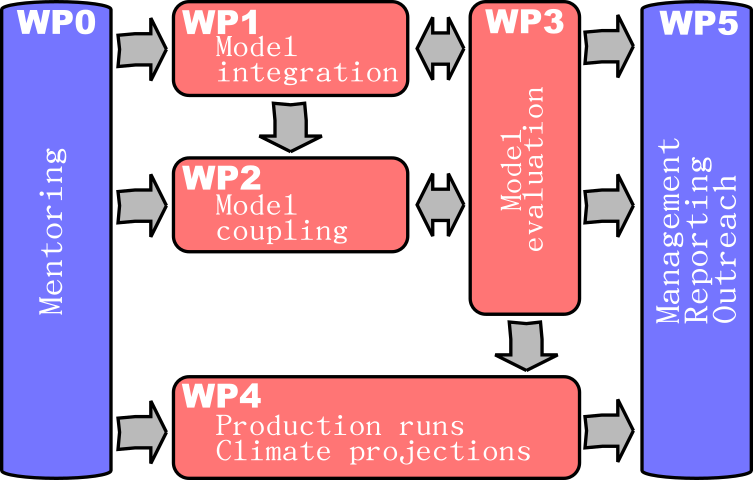
\includegraphics[width=0.48\linewidth]{wp_flow_chart}
  \label{fig:flowchart}}
  \subbottom[Gantt chart]{%
    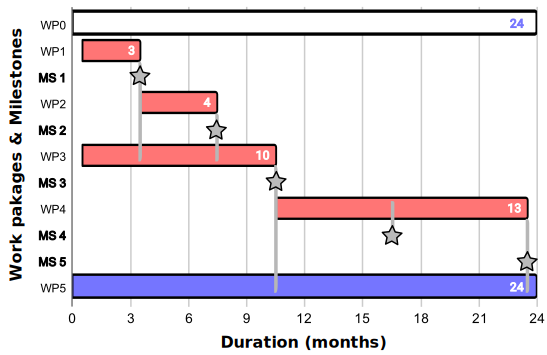
\includegraphics[width=0.48\linewidth]{gantt_chart}
  \label{fig:ganttchart}}
  \caption{\glspl{wp} as presented in this Section. \gls{wp}0 and \gls{wp}5 coordinate and communicate between the different \glspl{wp}m and therefore run during the whole duration of the project. Within \gls{wp}2 a three months research stay at \gls{ncar} lab in Boulder, COL, USA is planned. \gls{ms}~3 and 4 correspond to reporting to a funding agency (\gls{fwf}).
}
\end{figure}

\section{WP0 Management and mentoring}
\label{sec:wp0}
The management and mentoring \gls{wp}, as described above spans the entire project periode and includes a variety of bi-directional tasks in cooperation and with support of the faculty host and host institute at \gls{boku}. \gls{wp}0 is built upon the  core attributes of the Lise-Meitner fellowship  and shall enable the applicant to position herself as an emerging leader in land-atmosphere interactions, particularly the climate-vegetation-air quality nexus. During the start phase of the \gls{odina} project, \gls{wp}0 will ensure a smooth integration into the work environment at the host institute  and all aspects concerning technical, administrative and logistic support by the corresponding units of \gls{boku} (Task~0.1). The mid-phase is split into the development and honing of key skills for a future leadership role in Earth science (Task~0.2) and monitoring of the project progress (Task~0.3). Task~0.2 includes leadership and management training but also programs focusing on didactic skills, presentation techniques, public outreach formats, as well as contributions to  teaching and co-supervision of students. A detailed career development plan is presented in Section~\ref{sec:career}. In the end-phase \gls{wp}0 will initiate the preparation of follow-up proposals tailored to European and national funding schemes such as e.g. the \gls{fwf} Elise-Richter program or stand-alone projects (Task~0.4).

\subsection*{Work Package duration 24 months (months 1 to 24)}
\begin{enumerate}[start=1,label={T0.\arabic*}]
  \itemsep0pt
\item Getting started \hfill [month 1]
\item Career development \hfill [month 1 - 24]
\item Progress monitoring \hfill [month 1 - 23]
\item Follow-up projects \hfill [month 18 - 24]
\end{enumerate}

\section{WP1 Model integration}
\label{sec:wp1}
The model integration \gls{wp} will build on existing collaborations with technical and scientific staff at the \gls{uio} (Norway) and at \gls{ncar} in Boulder (USA) and include support by the scientific and technical team of the host institute at \gls{boku}, Vienna. Existing parts of the \gls{odina} model will be extended to describe our stateoftheart process understanding as accurately as possible. This will comprise
\begin{enumerate}
  \itemsep0pt
\item the inclusion of a state of stomata sluggishness,
\item to  consider a more explicit healing formulation for the \gls{odina} model (Task~1.1),  and
\item to deduce and update additional model parameters based on existing meta databases (Task~1.2).
\end{enumerate}
It is expected that the model output considering  active ozone damage will substantially differ between the updated (this proposal) and current model configuration (\gls{cmip}6). Initial cross-evaluation with data at global scales (coarse resolution model integration) and single site simulations (Task~1.3) following the \gls{cesm} standard procedures are likely to reveal the necessity for adjustment of additional free model parameters. In depth evaluation of individual parameters and results is subject to \gls{wp}3. In concert with \gls{wp}3 the \gls{wp}5 aims to present the  completed \gls{odina} model to the broad community on scientific meetings and within  a peer-reviewed model development paper (\gls{ms}~1 in Fig.~\ref{fig:ganttchart}).
\subsection*{Work Package duration 3 months (months 1 to 4)}
\begin{enumerate}[start=1,label={T1.\arabic*}]
  \itemsep0pt
\item Implementation of stomatal sluggishness and healing \hfill [month 1 - 2]
\item Deduction of additional parameters \hfill [month 2 - 3]
\item Initial model simulations and cross-evaluation \hfill [month 3 - 4]
\end{enumerate}

\section{WP2 Model coupling}
\label{sec:wp2}
Activities related to model coupling \gls{wp} will include a three month research stay at the \gls{ncar} lab in Boulder (USA) to both facilitate the technical work as well as build important networks for future work. A one-way coupling between the atmospheric chemistry component (e.g. \gls{cam}-chem) to the land-surface component (\gls{clm}) is achieved through the dry deposition implementation already in place in \gls{cesm}. The existing dry deposition scheme in \gls{cesm} will be evaluated concerning \gls{odina}. If necessary, the scheme will be improved and updated (Task~2.1). Two-way coupling will be achieved by propagating instantaneous ozone concentrations from the atmosphere through the coupler to the land component (Task~2.2). Technically this involves touching the model \gls{cesm} coupler infrastructure. The work on the coupling will be done in the most sustainable way during the planned research stay at \gls{ncar}. Potential infrastructure updates will be taken into consideration and integrated into the workflow. Initial tests and evaluation of the coupled model on coarse-grid global-scale as well as through  single site simulations are planned (Task~2.3). Detailed validation of the coupled model will be performed in coordination with \gls{wp}3 as in described in \gls{wp}1.

\subsection*{Work package duration 4 months (months 4 to 8)}
\begin{enumerate}[start=1,label={T2.\arabic*}]
  \itemsep0pt
\item Evaluation of the dry deposition scheme (improvement and update) \hfill [month 4 - 5]
\item Technically coupling \gls{cam}-chem ozone concentrations to \gls{odina} \\$\rightarrow$ research stay at \gls{ncar}/\gls{ucar} \hfill [month 5 - 6]
\item Perform model  tests of the coupling algorithm \hfill [month 6 - 8]
\end{enumerate}

\section{WP3 Model evaluation and update of model parameters}
\label{sec:wp3}
The evaluation of the updated model is an integral part of \gls{wp}1 and \gls{wp}2 and spans the whole duration of both \gls{wp}. Data for evaluation will be collected from FLUXNET sites with associated ground level ozone observations, e.g. \gls{airbase} (Task~3.1). Based on the collected data, the initial integration and validation tests are complemented and completed with more in depth evaluation for the selected sites (Task~3.2) and on global scales (Task~3.3). Model parameters  (e.g. $\mathrm{J_{max}}$0 in \gls{luna}, \glspl{pft}) will be adapted and adjusted for changes in the model baseline of, e.g. in terrestrial and vegetation carbon pools, inflicted ozone induced damage on photosynthesis and stomatal conductance (Task~3.4). A model evaluation paper after successful evaluation is pursued in coordination with \gls{wp}5 (\gls{ms}3). The model development and evaluation paper could be synthesized into one if necessary.

\subsection*{Work Package duration 10 months (months 1 to 11)}
\begin{enumerate}[start=1,label={T3.\arabic*}]
  \itemsep0pt
\item Collection of evaluation data \hfill [month 1 - 3]
\item Site level evaluation \hfill [month 3 - 6]
\item Global scale evaluation \hfill [month 6 - 11]
\item Update model parameters \hfill [month 3 - 11]
\end{enumerate}

\section{WP4 Production runs and climate projections}
\label{sec:wp4}
Upon successful implementation of \gls{wp}1-3 work on \gls{wp}4 is initiated. Within this final research work package production runs with climate projections will be performed. It is planned to perform at least one long term \gls{cmip} style ($1850-2100$) coupled model simulation (Task~4.1). As the highest tropospheric ozone abundances are expected for a low mitigation scenario with high anthropogenic greenhouse gas emissions and simultaneous substantial methane release from permafrost regions \parencites[e.g.][]{JGR:Rieder2015}{AE:Rieder2018}, thus \gls{ssp}~5 is selected as a future scenario. Additional simulations following other \glspl{ssp} are planned but depend on the workload at \gls{vsc} and thus cannot be guaranteed to be fully complete within the 24~month project timeline. Results will be compared with existing \gls{cmip}~6 reference simulations of \gls{cesm} to study the combined effects of climate and ozone feedback on vegetation in a coupled \gls{esm} (Task~4.2). Of special interest are implications on future surface ozone abundance and air quality indices along with induced plant damage and effects on the carbon cycle, e.g. expected reduction in \gls{gpp} with respect to reference simulations. The focus herein lies on populous and highly industrialized regions, e.g. Europe, East Asia, North America.

\subsection*{Work Package duration 13 months (months 11 to 24)}
\begin{enumerate}[start=1,label={T4.\arabic*}]
  \itemsep0pt
\item Run \gls{cesm} coupled of climatological timescales (\gls{ssp}5) \hfill [month 11 - 17]
\item Study climate and vegetation impact on surface ozone abundance \hfill [month 17 - 24]
\end{enumerate}

\section{WP5 Reporting and dissemination}
\label{sec:wp5}
\gls{wp}5 acts as an umbrella for reporting to the funding agency (\gls{fwf}) and dissemination to scientific and lay audiences. \gls{wp}5 spans the whole project duration and is effectively the coordinating and reporting hub for \gls{wp}1--4. Science communication (Task~5.1) is further divided into publications, e.g. research papers, conference contributions, and public outreach. Public outreach will include among others contributions to popular science blogs or presentations to the general public. Dissemination using social media platforms such as twitter will be considered if applicable. In close interaction with \gls{wp}0 and under guidance by the host institution, targeted networking activities are planned (e.g. conferences, workshops, professional networks) (Task~5.2). The submission of the final report to the funding agency (\gls{fwf}) is officially concluding \gls{wp}5 (Task~5.3) although several additional papers are expected to emerge from the project results which will be submitted past official completion.

\subsection*{Work Package duration 24 months (months 1 to 24)}
\begin{enumerate}[start=1,label={T5.\arabic*}]
  \itemsep0pt
\item Science communication \hfill [month 3 - 24]
\item Networking \hfill [month 1 - 24]
\item Submit final report  to funding agency (\gls{fwf}) \hfill [month 23 - 24] \textbf{\color{red}TODO: Abklaeren, wann dieser faellig ist.}
\end{enumerate}
